\documentclass[a4paper,parskip]{scrartcl}
\usepackage[usenames,dvipsnames,svgnames,table]{xcolor}
\usepackage[utf8]{inputenc}
\usepackage[ngerman]{babel}
\usepackage{amsmath}
\usepackage{enumerate}
\usepackage{textcomp}
\usepackage{fancyhdr}
\usepackage[a4paper]{geometry}
\usepackage{amsthm}
\usepackage{amsfonts}
\usepackage[version=3]{mhchem}
\usepackage{graphicx}


\author{Sven Jandura \& Edward Wang} 
\title{Auswertung des Versuchs H2}

\geometry {
  top=0.75in,
  headsep=3ex,
  bottom=0.75in,
}

\fancypagestyle{plain}{
  \fancyhf{}
  \fancyhead[L]{Sven Jandura \& Edward Wang}
  %\fancyhead[C]{} %Center
  \fancyhead[R]{Seite \thepage}
}

\renewcommand{\headrule}{\color{Black}\hrule height\headrulewidth\hfill}
\pagestyle{plain}

\let\stdsection\section\renewcommand\section{\newpage\stdsection}

\newtheorem{mydef}{Definition}
\newtheorem{mythe}{Satz}


\begin{document}

\maketitle

\tableofcontents

\section{Ziel}

Ziel dieses Versuchs ist die experimentelle Messung der D2-Linie im Rubidium.

\section{Grundlagen}

In der Quantenmechanik werden die Elektronenorbitale von Atomen durch diskrete Energieniveaus beschrieben. Dabei kann es zu Übergänge zwischen diesen Zuständen kommen, bei denen ein Photon absorbiert bzw. emittiert wird. Die Frequenz dieses Photons wird dann gemäß der Planck-Formel durch $E_2 - E_1 = h \nu$ gegeben. Durch Messung dieser Resonanzfrequenz $\nu$ kann man die Abstände der Energieniveaus bestimmen. Allerdings lässt sich diese Spektrallinie nicht beliebig scharf messen, sondern sie besitzt eine gewisse Linienbreite. Grund dafür sind, u.a., die Stoßverbreiterung, die durch Wechselwirkungen zwischen verschiedenen Atomen verursacht wird, die Dopplerverbreiterung und die natürliche Linienbreite. Die natürliche Linienbreite kommt dadurch zustande, dass diese angeregte Zustände nur kurzlebig sind, und wegen der Energie-Zeit-Unschärfe ist die Energie dieses angeregten Zustandes also nicht genau definiert. Die Linie nimmt die Form eines Lorentz-Peaks:
\begin{equation}
    I(\omega) = I_0 \frac{1}{\pi} \frac{\gamma/2}{(\omega - \omega_0)^2 + (\gamma / 2)^2}
\end{equation}
Die Doppler-Verbreiterung entsteht wegen der statistischen Geschwindigkeitsverteilung der Teilchen im Gas. Dadurch kommt es zu einer Doppler-Verschiebung des Lichts, gemäß
\begin{equation}
    \omega' = \omega_0 \left(1 - \frac{v_z}{c} \right)
\end{equation}
Somit berechnet sich die absorbierte Intensität zu einem Gauß-Peak:
\begin{equation}
    I(\omega) = I(\omega_0) e^{- \left( \frac{\omega - \omega_0}{\delta \omega_D/\sqrt{4 ln 2}} \right)^2}
\end{equation}
wobei
\begin{equation}
    \delta \omega_D = \frac{\omega_0}{c} \sqrt{\frac{8 kT ln2}{m}}
\end{equation}

Das Rubidium-Atom besitzt nur ein Valenzelektron, d. h., die inneren Schalen sind abgeschlossen und tragen nicht für den Gesamtdrehimpuls bzw. Spin bei. Außerdem kann man die Wechselwirkungen zwischen dieses Valenzelektron und die restlichen vernachlässigen, weshalb es als wasserstoffähnlich bezeichnet wird. Wir betrachten die beiden Isotope Rb-85 und Rb-87, die stabil sind, und dessen Kernspins jeweils $5/2$ bzw. $3/2$ beträgt. Wir berücksichtigen zum einen die Grobstruktur, die durch den Abstand der Elektronen zum Kern ensteht, die Feinstruktur, in der die Spin-Bahn-Kopplung berücksichtigt wird, d.h. die Wechselwirkung zwischen den von dem Spin und dem Bahndrehimpuls erzeugten magnetischen Momenten, und die Hyperfeinstruktur, bei der die Kopplung zwischen den Gesamtdrehimpuls und den Kernspin betrachtet wird.

Somit spaltet sich die D2-Linie, die durch den Übergang zwischen den $5^2s_{1/2}$ und den $5^2p_{3/2}$ Zuständen erzeugt wird, in 6 Linien auf.

\section{Versuchsdurchführung}

\subsection{Absorptionsspektroskopie}

 Bei der Absorptionsspektroskopie messen wird das transmittierte Licht durch das Rubidium-Gas. Dabei erwarten wir, dass bei der Durchstimmung der Laserfrequenz eine Senkung der transmittierten Intensität bei den Übergangsfrequenzen beobachtet wird. Das Experiment wurde so aufgebaut, dass ein Laserstrahl durch ein Prismenpaar geschickt wird, damit er rund wird, dann durchquert er ein $\lambda /2$ Plättchen und einen polarisierenden Strahlteiler, die Rubidium-Zelle, und wird schließlich durch eine Linse in die Photodiode fokussiert, wo dann die Intensität des Lichts gemessen wird. Der reflektierte Teil im Strahlteiler wird in einem Referenzresonator der Länte 10cm geleitet, damit man den freine Spektralbereich nach 
\begin{equation}
	\Delta \nu = \frac{c}{2d}
\end{equation}
bestimmt werden kann.
Ein Funktionsgenerator durchstimmt den Laser mit einer Frequenz von ca. 20 Hz und die Intensität wird mit einem Oszilloskop gespeichert.

\subsection{Sättigungsspektroskopie}

Ziel der Sättigungsspektroskopie ist es, die Dopplerverbreiterung zu vermeiden. Dabei ist der Unterschied zur Absorptionsspektroskopie, dass der Strahl die Zelle zweimal in umgekehrten Richtungen durchquert. Experimentell wird es umgesetzt, indem der linear polarisierte Strahl nach der Rubidium-Zelle durch einen ND-Filter abgeschwächt wird, durch ein $\lambda/4$ Plättchen zirkular polarisiert, in einem Spiegel reflektiert und wieder linear polarisiert wird, bevor er die Rubidium-Zelle nochmal durchläuft. Bei der Reflektion wird die zirkulare Polarisation umgedreht, sodass der Teststrahl nach der $\lambda/4$ Platte senkrecht zum Pumpstrahl polarisiert ist, und deshalb beim polarisierenden Strahlteiler komplett in der Diode reflektiert wird. Auch hier wird der Strahl durch eine Linse fokussiert.

Bei diesem Versuch erwarten wir die selben Senkungen zu beobachten, wie in der Absorptionsspektroskopie, allerdings mit sogenannten Lamb-Dips. Wenn der Pumpstrahl die Resonanzfrequenz eines Übergangs trifft, regt er Atome im Gas an, und wenn diese Atome entlang der Verbreitungsachse des Strahls eine Geschwindigkeit nahe Null haben, wird aus Sicht dieser Atome der Teststrahl die selbe Frequenz besitzen wie der Pumpstrahl; allerdings können sie nicht durch den Teststrahl angeregt werden, da diese Anregung schon durch den Pumpstrahl gesättigt wurde. Somit entstehen Peaks im Intensitätsprofil.

\section{Absorbtionsspektrum}

Es wird werden die Peaks des Referenzresonator gegen die Zeit aufgetragen und mit einem Polynom dritter Ordung gefitted, um die Nichtlinearitär der Verstimmung des Lasers zu korrigieren.

\begin{figure}[h]
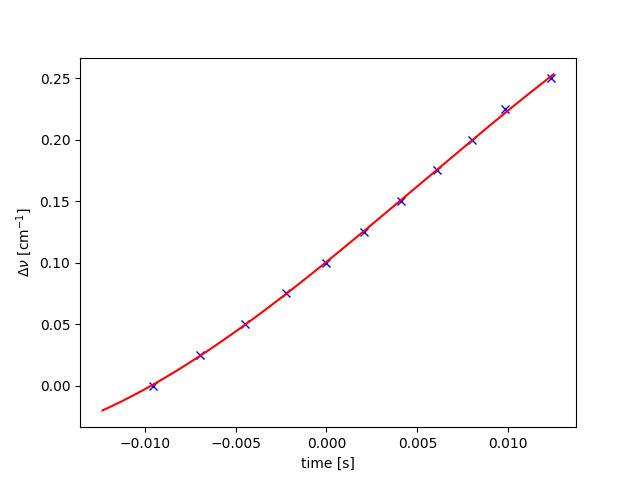
\includegraphics[scale = 0.5]{./absorbtion/frequencyCorrection}
\end{figure}

\end{document}
